\begin{exercise}
Verify that the following two results---known as the Pullback Lemmas---are
a consequence of \partref{1}{1}{4}{ii} and \partref{1}{1}{4}{iii} in the previous exercise.
Consider
\begin{equation*}
\begin{tikzcd}[row sep=small, column sep=small]
\bullet \arrow[rr] \arrow[dd] && \bullet \arrow[rr] \arrow[dd] && \bullet \arrow[dd] \\
& (\mathrm{B}) && (\mathrm{A}) \\
\bullet \arrow[rr] && \bullet \arrow[rr] && \bullet \\
\end{tikzcd}
\end{equation*}
\begin{parts}
\part
If \((\mathrm{A})\) and \((\mathrm{B})\) are pullback squares, then the outer rectangle is also a pullback square.
\part
If the outer rectangle and \((\mathrm{A})\) are pullback squares, then \((\mathrm{B})\) is a pullback square as well.
\end{parts}
\end{exercise}

\begin{solution}
Recall (e.g., from \cite[Proposition~1.1.6(ii)]{MR1674451}) that in a category \(\cat{B}\), a commutative square
\begin{equation*}
\begin{tikzcd}
X \arrow[r, "f"] \arrow[d, "p"] & Y \arrow[d, "q"] \\
I \arrow[r, "u"] & J
\end{tikzcd}
\end{equation*}
is a pullback square if and only if \((u, f)\) is a Cartesian lift of \(u\) in the context of the codomain functor \(\cod : \cat{B}^{\rightarrow} \to \cat{B}\), as in the following diagram.
\begin{equation*}
\begin{tikzcd}
\begin{pmatrix}
\begin{tikzpicture}
        \node(1){\(X\)}; 
        \node(2)[below of=1]{\(I\)};
        \draw[->](1)--node[right]{\scriptsize\(p\)} (2);
\end{tikzpicture}
\end{pmatrix}
\arrow[r, "{(u, f)}"] \arrow[d, -Triangle, "\cod"]
&
\begin{pmatrix}
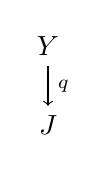
\begin{tikzpicture}
        \node(1){\(Y\)}; 
        \node(2)[below of=1]{\(J\)};
        \draw[->](1)--node[right]{\scriptsize\(q\)} (2);
\end{tikzpicture}
\end{pmatrix} \arrow[d, -Triangle, "\cod"]
\\
I \arrow[r, "u"] & J
\end{tikzcd}
\end{equation*}
Therefore, \partref{1}{1}{5}{i} and \partref{1}{1}{5}{ii} follow immediately from \expartref{1}{1}{4}{ii} and \expartref{1}{1}{4}{iii}, respectively.
\end{solution}